% !TEX encoding = UTF-8 Unicode
\documentclass{report}

\title{Practical IT-Security: CSRF}
\author{Michael Müller}
\date{\today}
	
% big font for sections
\usepackage{sectsty}
\sectionfont{\LARGE}

\usepackage{graphicx}
\usepackage{wrapfig}
\usepackage{caption}
\usepackage{subcaption}
\usepackage{listings}
\usepackage{hyperref}

% \begin{comment} ... \end{comment{}
\usepackage{verbatim}

\setlength{\parskip}{0pt}

\makeatletter
\renewcommand{\paragraph}{
  \@startsection{paragraph}{4}
    {\z@}{1.25ex \@plus 1ex \@minus .2ex}{-1em}
      {\normalfont\normalsize\bfseries}
      }
      \makeatother


\begin{document}

\newpage

\maketitle

\newpage


%=================
\section{Introduction}

Cross-Site-Request-Forgery (\textsc{CSRF}) is an attack on web-applications
which will be further explained within the presentation.
This document is meant as a preparation document in order to get you ready to
understand the presentation and conduct the assignments.

\begin{comment}
\subsection{HTTP}
The HTTP protocol is the driving force behind the web.

\subsubsection{GET}
foo ar



\begin{lstlisting}[
	caption=Typical HTTP GET request
]
GET / HTTP/1.1
Host: google.com
\end{lstlisting}

\begin{lstlisting}[
	caption=Typical HTTP GET reply
]
200 OK 
\end{lstlisting}

\subsubsection{POST}
\end{comment}


%=================
\subsection{Web Developer Tool}

We aim to exploit several web-services in the assignments. Most of the 
exploits will be written in HTML in conjuction with JavaScript. For this 
purpose it comes handy if you are familiar with the developer tool of your 
favorite webbrowser.
Most modern browsers come with some kind of developer tool. Check the
corresponding manual or install a fitting plugin like Firebug (for Firefox). 
For Chromium the developer tools are accessible via ``Tools > Developer 
Tools'' (or via pressing F12).
The main features of the developer tools, which will come handy for us, are: 

\paragraph{The JavaScript Console}
Comes handy when debugging JavaScript code, since execution errors are
displayed and you have the ability to interactively execute code on the
webpage.
\begin{figure}[h!]
	\centering
	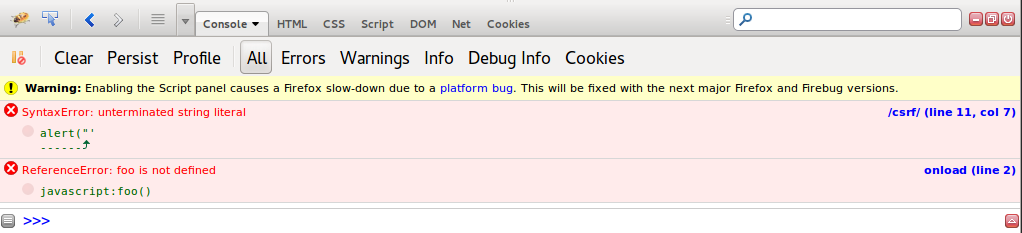
\includegraphics[width=1.0\textwidth]
		{./images/jsconsole.png}
	\caption{
		Firebug JavaScript console.
	}
	\label{fig:jsconsole}
\end{figure}

\paragraph{The Network Capturer}
Enables you to analyze and debug HTTP requests/replies which are send/received 
by the browser. Of course, you can also use Wireshark or similar tools as
means to capture HTTP traffic. From my experience, however, it comes handy to
use the builtin browser tools, since they oftentimes are nicely
integrated and tie in well with the HTML/JavaScript coding workflow.
\begin{figure}[h!]
	\centering
	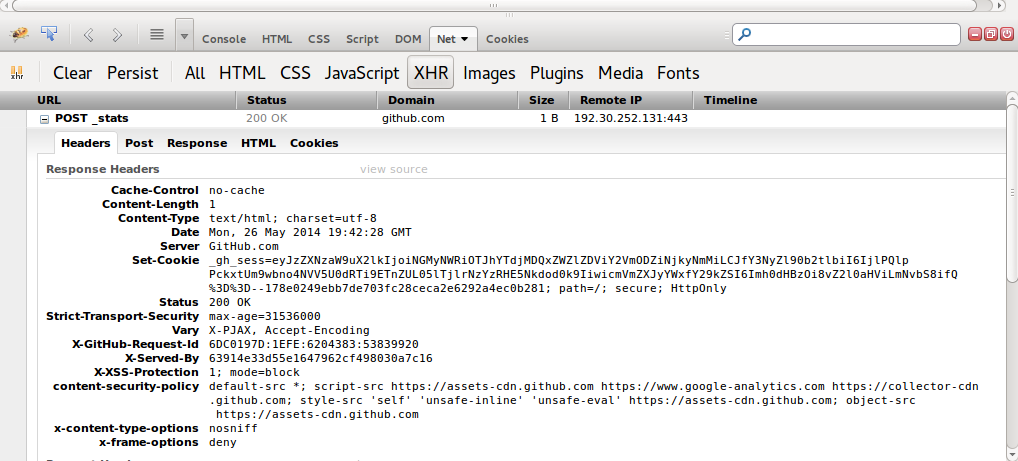
\includegraphics[width=1.0\textwidth]
		{./images/httpcapturer.png}
	\caption{
		Captured HTTP traffic within Firebug.
	}
	\label{fig:httpcapturer}
\end{figure}

\begin{comment}
\paragraph{Disabling the Cache}
\begin{figure}[h!]
	\centering
	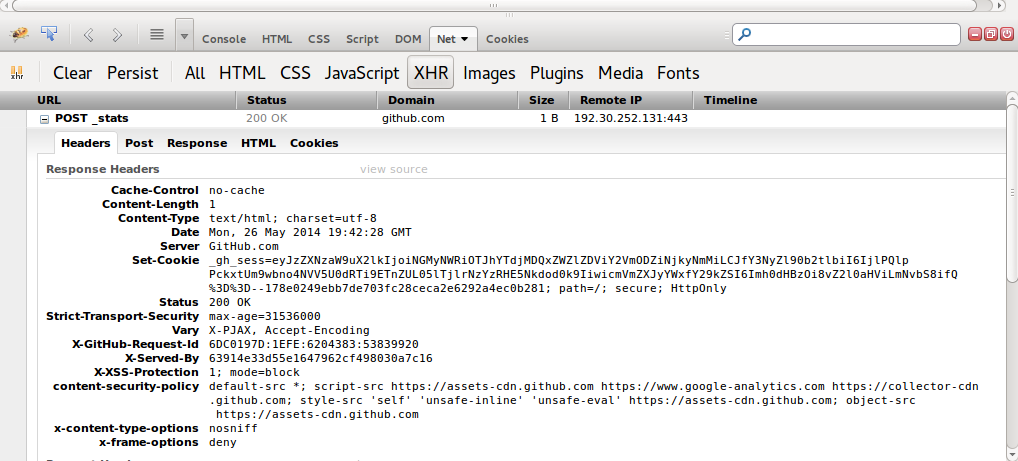
\includegraphics[width=1.0\textwidth]
		{./images/httpcapturer.png}
	\caption{
		Firebug captures HTTP traffic.
	}
	\label{fig:httpcapturer}
\end{figure}
\end{comment}


%=================
\newpage
\section{Assignments}

To carry out the assignments you need to bring your own laptop configured
to the run the services described in this section.

\subsection{Metasploitable}
We will continue to use the Metasploitable image, which has been provided 
in the warm-up phase of the course. If you no longer have it at hand you
could download it from the 
\href{https://moodle.uni-ulm.de/course/view.php?id=1312}{Moodle} platform
again. 

Use a virtualisiation software to get the image running as a virtual 
machine (vm). The VirtualBox software works well, for example. Configure 
the vm in a way that you have access to it over network (e.g. by configuring 
a Bridged Adapter within VirtualBox). If network access does not work out 
of the box you may have to log into Metasploitable (User: \texttt{msfadmin}, 
Password: \texttt{msfadmin}) and execute ``\texttt{\$ sudo dhclient eth0}'' 
in order to obtain an IP address.

If everything worked out, you should be able to access the Metasploitable 
webserver from your host machine. If the vm e.g. runs on 192.168.1.103,
the address would be \href{http://192.168.1.103/}{http://192.168.1.103/}.

\subsubsection{Damn Vulnerable Web App}
If you have not already done so in the warm-up phase of the course,
you should now log into the web application in order to get a feeling for 
the interface.
Open up \href{http://metasploitable-vm-ip/dvwa}{http://metasploitable-vm-ip/dvwa}
and log-in with the credentials User: \texttt{admin}, Password: 
\texttt{password}.
Open the navigation tab ``DVWA Security'' and configure ``Security Level: Low''
(see Figure \ref{fig:dvwa0}).

During the assignments we will work our way through the security levels 
low and medium. The level high is meant to show 
the state of art of a best-practice solution. It is not meant to be cracked.\\

\textbf{Note:} The security level which you configure is saved as a Cookie 
value. The default value is high. This might lead to problems
while debugging: if you e.g. log into DVWA using Chromium and configure
low you should also run your exploits in Chromium and not 
in e.g. Firefox. Firefox would still be configured for the security level
high.

\begin{figure}[h!]
	\centering
	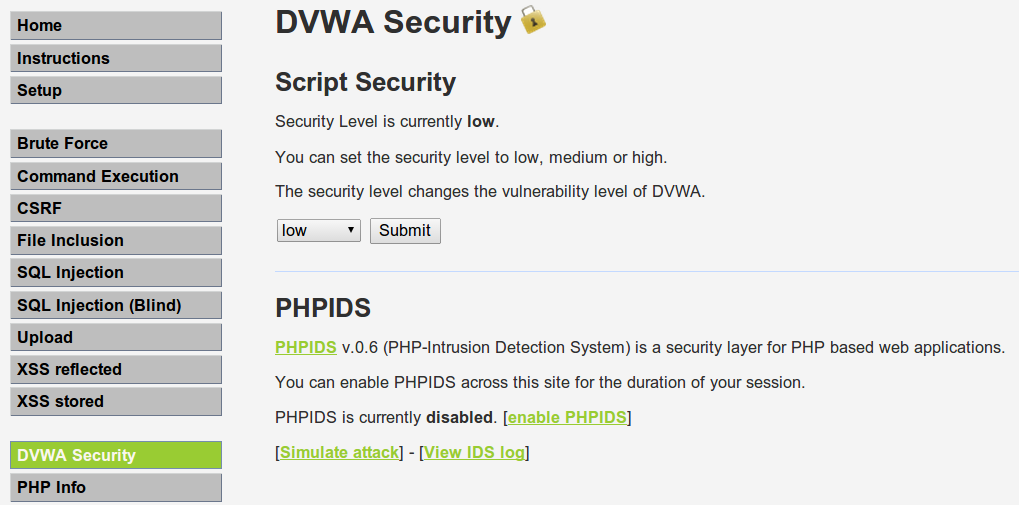
\includegraphics[width=0.8\textwidth]
		{./images/dvwa-security.png}
	\caption{
		Beware! The security level is only set temporarily as a
		Cookie!
	}
	\label{fig:dvwa0}
\end{figure}

\subsubsection{TWiki}
The other Metasploitable service which we will examine is TWiki. If the
Metasploitable image is running you can access the application via 
\href{http://metasploitable-vm-ip/twiki}{http://metasploitable-vm-ip/twiki/}.

\subsection{advanced-csrf}
The advanced-csrf package is a simple web application designed
to be exploitable for CSRF/XSS attacks. 
You will obtain a link to an archive with the PHP code and a MySQL dump
at the start of the assignments. The application requires a WebServer with 
PHP v.5.x support and a MySQL v.5.x database in order to run.
%To install the package extract the package into a folder which
%is configured to contain PHP code.

The easiest way to run the application is to set up a local webserver. A 
comfortable way of doing so is to use 
\href{https://www.apachefriends.org/index.html}{XAMPP}, an
environment which comes with a webserver and provides pre-configured PHP 
and MySQL support.

%After successful installation of a webserver point your browser to 
%\href{http://localhost/advanced-csrf/index.php}
	%{http://localhost/advanced-csrf/index.php}. You should
%see a webpage similar to the one in Figure \ref{fig:ace} 
%there (todo: add figure).


%==========================
%\newpage
\section{Quick Checklist}

If you have encountered errors within the previous steps or have any questions
regarding the assignments you can contact me via
\href{mailto:michael-4.mueller@uni-ulm.de}{michael-4.mueller@uni-ulm.de}. 
To give a quick, summarized overview of the requirements for the assignments:

\begin{comment}
The course will roughly be structured in this way:

\begin{tabular}{{l}{l}}
09.00-09.50	& Presentation CSRF\\
09.50-10.00	& Short Pause / Preparation for the assignments\\
\ \\
10.00-10.30	& Assignment 1\\
10.30-10.40	& Presentation Solution\\
\ \\
10.40-11.40	& Assignment 2\\
11.40-12.00	& Presentation Solution\\
\end{tabular}
\end{comment}


\paragraph{You should bring a basic understanding of}
\ \\
HTTP, HTML, the DOM, PHP, JavaScript and JSON. 
We won't dive deep into markup or language subtleties, but you should have
a basic understanding. 
It would be a pity if you would spent a lot of effort fiddling on syntax 
particularities, so don't be afraid to ask me if you get stuck.

The DVWA offers the possibility of displaying the (PHP) code of the
web page which you are trying to exploit. A basic understanding of
PHP may come in handy here. 

Some of the assignments make use of the jQuery framework. You don't need to
have an in-depth understanding of the framework, but it will make the
assignments easier for you if you understand that certain syntax belongs to
the framework




\paragraph{You should bring}
\ \\
A laptop. Configured to run the Metasploitable virtual machine. The
advanced-csrf web application should be able to run as well 
(requires PHP v.5.x and MySQL v.5.x).

\paragraph{You should have played with}
\ \\
A tool to capture HTTP requests/replies of your webbrowser and a JavaScript 
console, which displays execution errors.

\paragraph{You should be willing}
\ \\
To enjoy learning something new and nibble on puzzles.

\center
\ \\
\texttt{\$ ./happy\_hacking -\--from 1401865200000 -\--to 1401876000000 -\--at "O27 / 341" -\--mood ":)"  }

\end{document}
